% \documentclass[review]{elsarticle}
\documentclass[final,3p,times,onecolumn,sort&compress]{elsarticle}

\usepackage{lineno,hyperref}
\usepackage{listings}
\usepackage{subcaption}
\modulolinenumbers[2]

\usepackage{array}
\newenvironment{conditions}
  {\par\vspace{\abovedisplayskip}\noindent\begin{tabular}{>{$}l<{$} @{${}={}$} l}}
  {\end{tabular}\par\vspace{\belowdisplayskip}}
\newcolumntype{R}{>{\raggedleft\arraybackslash}m{2cm}}


\lstset{language=Python,
    basicstyle=\footnotesize\ttfamily,
    % commentstyle=\ttfamily\itshape\color{gray},
    stringstyle=\ttfamily,
    showstringspaces=false,
    breaklines=true,
    frameround=ffff,
    frame=single,
    % rulecolor=\color{black},
    tabsize=1,
    % keywordstyle=\color{red}\bfseries,
    columns=fullflexible,
    morekeywords={public, class}
    morecomment=[s]{"""}{"""},
}

\journal{ }

%% Elsevier bibliography styles
%% APA style
\bibliographystyle{model5-names}\biboptions{authoryear}

%%%%%%%%%%%%%%%%%%%%%%%

\begin{document}

\begin{frontmatter}

\title{Measuring inequality in the built environment: Evaluating grocery store access for planning policy and intervention}

% \author[]{T M Logan\corref{mycorrespondingauthor}}
% \ead{tom.logan@canterbury.ac.nz}
% \author[]{M J Anderson}

% \address{Civil and Natural Resources Engineering, University of Canterbury, New Zealand}

\begin{abstract}
The built environment has institutionalized many of the inequities prevalent in our society.
<something's missing here>
While inequity and inequality are often evaluated for income, there are many other goods, services, and also undesirable quantities (such as exposure to environmental harm) that are distributed throughout our communities.
To understand and address inequity in how these quantities are distributed, we need to measure and identify inequality.
To go beyond equality, we need the ability to evaluate inequality between subgroups within our communities.
However, existing approaches to evaluating the equality of distributions are insufficient or, in the case of undesirable quantities, mathematically unsuitable.
Recently, in the risk science literature, a quantitative measure for the performance and inequality of a distribution was presented for evaluating the equality of health risk.
In this paper, we demonstrate how this measure (which uses the \textit{equally-distributed equivalent}: EDE) and associated index could be used in an urban planning and hazard contexts to support decision making to foster equity in the built environment.
We use examples of food access in cities across the USA and post-hazard recovery as illustrations.
\end{abstract}

\begin{keyword}
Urban planning $|$ Equity $|$ Environmental justice 

\end{keyword}

\end{frontmatter}

% \linenumbers

\section{Introduction}
As our cities undergo the major and rapid changes prompted by climate change, population growth, the urban renaissance, and the pandemic response, the distributions of environmental burdens and amenities will shift.
As alternative interventions are discussed, there are two objects that need to be considered.
The first is that we ensure people's exposure to burden is minimized and their access to resources is maximized.
The second, is that the distribution of these burdens and resources must be fair.
This fairness is critical for community trust and cohesion, which is necessary for community sustainability and resilience \citep{Dempsey2011-og, Cutter2008-NJ, Logan2020-vj}.
Thus, there is a global and time-critical imperative to improve the distribution of environmental resources and burdens.
To deliver optimal and fair allocations, planners, policy makers, designers, and engineers need the ability to evaluate scenarios, through the lens of equity, in a substantive manner.

How we design our communities and react to hazards, drives how burdens and resources are distributed between our people \citep{Wilson2008-yk}.
These burdens include exposure to air pollution \cite{Maguire2011-fi, Sheriff2020-ge}, natural hazards \citep{Burby2000-qe, Saunders2007-of}, hours spent commuting \citep{Frumkin2004-yi}, and chronic diseases \citep{Lopez2006-jb}.
Resources, many of which ameliorate some of these burdens, include trees \citep{Schwarz2015-fs} and amenities like supermarkets, schools, health care, and green space \citep{Logan2019-fr, Nesbitt2019-sk, Pacione1989-ui, Apparicio2007-di, Whitehead2019-tf}.
For example, access to healthy food improves peoples' diets, which improves their health \citep{Garcia2020-xt, Kolak2018-az}.
Whereas green space mitigates flooding, heat, erosion, and air pollution, while providing opportunities for recreation, improved mental health, and the forging of social capital \citep{Dempsey2011-og, Astell-Burt2013-og,Kazmierczak2011-ot, Norton2015-vv}.
Unfortunately, empirical evidence consistently reveals that these burdens and resources are not equally distributed among people;
globally, across scales and disparate contexts, disadvantaged and underprivileged people are systematically exposed to larger environmental burdens and have less access to beneficial resources.
The future threatens to increase these disparities.

Fairness, and what it constitutes, is characterized by the concepts of equality, equity, and environmental justice \citep{Talen1998-mk, Low2013-yx, Rigolon2019-zr, Lopez2011-cc}.
In this paper, we consider equality to be homogeneity in the amount of a resource distributed to the recipients, whereas equity is distribution based on need \citep{Talen1998-mk, Lucy1981-xr}.
For example, \cite{Rumley2014-pu} provided the anecdote that giving two children each an apple achieves equality; however, this is not equitable if one child has not eaten in three days. 
In turn, environmental justice --- the notion that everyone has the right to a healthy environment \citep{Lopez2011-cc} --- is achieved through equity in distributional, procedural, and interactional justice \cite{Low2013-yx}.
Distributional justice is influenced by where we place resources and guide residential development.
How we create spaces influences interactional justice, as approaches such as mixed-use design encourage a diversity of users and enables people to interact safely \citep{Jacobs1961-po}.
And whether communities are empowered and engaged during the decision-making process has an influence on procedural justice \citep{Low2013-yx, Rigolon2019-zr}.

To guide the decision-making process by evaluating policies and interventions, we need a substantive measure of a distribution, that penalizes for inequality.
This measure must reflect the realized value of the distribution, rather than solely a relative index of variation as, in spatial planning, some degree of geographic inequality is inevitable given some people inherently (e.g.,) live closer to a resource \citep{Dadashpoor2016-ar, Nesbitt2019-sk}.
Additionally, this measure must be able to consider the equality between subgroups, as some groups within our communities simply need more of some resources than others.
For example, youth need access to schools, while older people need a higher access to health care \citep{Syed2013-aj}.
Older people, at risk of social isolation, also need higher access to green space where they can build their social capital \citep{Frumkin2004-yi}
Additionally, groups with increasing rates of obesity (women, racial-minorities, and low-income communities \citep{Day2006-ak}) need improved access to healthy food outlets \citep{Garcia2020-xt, Kolak2018-az} and environments that promote physical activity \citep{Krenichyn2006-ve}.
Finally, minority groups who were subject to discriminatory housing policies over 50 years ago are still experiencing the consequences with high rates of unemployment and chronic disease \citep{White2020-red}.
In practice, this type of analysis often means beginning with an assessment of equality, which is then coupled with an evaluation of need, based on socioeconomic information \citep{Talen1998-mk, Whitehead2019-tf, Schwarz2015-fs, Harlan2006-ap}.
% This evaluation of need accounts for the various subgroups, assesses whether they have been traditionally marginalized, or do not have the capacity to compensate for the amount of burden or resources they face \citep{Talen1998-mk, Whitehead2019-tf, Schwarz2015-fs, Harlan2006-ap}.
Understanding, visualizing, and quantifying how resources are allocated and the fairness of distributions is a significant tool for supporting decision-makers to incentivize development to ensure the future changes are both widely beneficial and fair. 

However, existing measures of inequality have had major limitations that have restricted their utility in urban planning. 
Fortunately, those limitations have been addressed by a recently proposed measure of equality --- the Kolm-Pollak method \citep{Sheriff2020-ge} --- and this, we believe, has enabled numerous opportunities for planners.
The objective of this paper is to demonstrate how this Kolm-Pollak approach can be used in a planning context to provide a substantive measure of evaluating interventions based on both the overall utility and effect on equity.

\section{Measuring equality in the built environment}
The built environment influences both distributional and interactional equity; that is, how burdens and resources are located and how urban form fosters safety and diversity (e.g., \cite{Jacobs1961-po, Low2013-yx}). 
However, the majority of studies focus on distributional equity (with some exceptions e.g., \cite{Williams2020-greenspace}).
The approaches used include equity mapping, regression and correlation analysis, cluster analysis, and distributions or summary statistics.

Equity mapping and other map-based visualization approaches are irreplaceable as they identify the specific regions lacking in or over exposed to the quantity in question \citep{Talen1998-fl, Wolch2005-wz}. 
Maps are also essential for supporting decision-makers and residents appreciate the geographic arrangement of resources and enable them to visualize how the locations can result in disparities distribution \citep{Talen1998-fl}.

Regression and correlation approaches are also commonly used to investigate equity (e.g., \cite{Schwarz2015-fs, Nesbitt2019-sk, Kim2016-mc, Williams2020-greenspace, Apparicio2007-di}).
These approaches are investigating whether there are consistent disparities based on any of the socioeconomic factors considered.

Another common analysis for amenity provision, is using spatial clustering and correlation approaches.
The foremost approach is \cite{Anselin1995-fh}'s Local Indicators of Spatial Autocorrelation (LISA). 
Similar to the regression approaches, LISA assessing the relationship between some quantities distribution and other, often socioeconomic, variables \citep{Talen1997-gl, Smoyer-Tomic2004-eh,Garcia2020-xt}.
An alternative clustering type technique is the Mann-Whitney U test, which assesses the difference between a geographic unit and its neighbors and determines the significance of this difference \citep{Nicholls2001-pf}.

The remaining approaches relate to summary statistics and are used to describe an entire distribution; which is what this paper will focus on.
Quantitative summary measures can complement map-based approaches, as they are necessary to support analysis such as ranking of interventions, ranking of cities for allocating assistance, or for optimization in a manner that visualizations are unable to support (e.g., Figure \ref{fig:the_challenge}).
Summary statistics are generally categorized as a measure of a distribution's dispersion (aka. the spread or variation), it's central location (i.e., its approximate value), or a measure of position (e.g., the quantiles).
For example, simple summary statistics for the central location include the mean/average and the median.
Well known summary statistics for the dispersion include the standard deviation, the variance, and the range.
Popular measures of equality tend to be drawn from the dispersion statistics, notably the Gini coefficient, and the coefficient of variation.
Another common measure, the percentage of people within some threshold value, is a measure of position.
However, these existing measures are either unsuitable or can introduce substantial error \citep{Kolak2018-az,Logan2019-fr}.
\newline

\begin{center}
[here we could have a figure showing a histogram and the mean, the standard deviation, the percentage within some threshold, highlighting the challenges of those measures.]
\newline
\end{center}

Consider Figure 1, a histogram showing the distribution of a resource between residents.
In this example we are showing how distance to the nearest supermarket is distributed among residents in Houston. 
If we only consider a measure of central location (the mean) or the percentage of people who live within some distance threshold (a measure of position), then we ignore the tail end of the distribution: the residents who are worst-off.
Alternatively, if we consider a measure of dispersion such as the standard deviation, then we consider the relative dispersion, at the omission of considering the true values. 
Considering relative values may be useful when comparing the wealth distributions countries with varying value of money.
However, in situations of interest to planners and city engineers, the absolute value of a distribution matters and it is plausible that a less equal distribution may be the more desirable in some instances.
For example, in a hazards context, a situation in which everyone is equally majorly affected by an event is likely less desirable than one where some residents are not impacted while the others are slightly effected, even though this latter case is less equal.

Nevertheless, measures of dispersion with these limitations are commonly used to measure equality.
The Gini coefficient, is the most commonly used \citep{Whitehead2019-tf, Maguire2011-fi}, and is a measure of dispersion.
It measures the difference between the distribution and if everyone were receiving the exact same value (``perfect'' equality). 
The coefficient of variation is another measure of dispersion, as it is the standard deviation normalized by the mean. 
It was first used in the assessment of school locations \citep{Pacione1989-ui}.

In addition to their inability to represent the location of a distribution, these measures of dispersion are also unsuitable or unsatisfactory for measuring equality as a desirable concept \citep{Maguire2011-fi, Atkinson1970-mr, Adger1997-tu}.
Both measures are `positive,' meaning they require no value judgement, they simply represent the dispersion of a distribution and are indifferent to whether that inequality is at the top or bottom of the distribution.
Essentially, these statistical measures of dispersion do not prioritize improving the state of the `poorest' individuals.

To address these limitations, \cite{Atkinson1970-mr} proposed using an equally-distributed equivalent (EDE).
This is a measure of both the central location of a distribution, which is penalized for inequality based on a social welfare function. 
An EDE represents the value which would, if everyone had that same value, provide the same level of welfare as the existing distribution.
An EDE is analogous to the risk premium or certainty equivalent from decision science and is, in practice, an alternative summary statistic for a distribution that captures both the location (c.f. the mean or median) and the dispersion (c.f. the variance) of a distribution.  
Unlike other `positive' summary statistics, however, the EDE is based on a subjective parameter that represents aversion to inequality and is how welfare is determined.
The use of this parameter shifts the value judgment regarding the importance of inequality from being implicit, as it is for the Gini coefficient and coefficient of variation, to being explicit and user defined.
While some users are uncomfortable with the subjectivity of a user-defined parameter, this is a somewhat false criticism, given that the act of choosing an alternative measure is to also make a value judgement regarding the user's aversion to inequality. 
Instead, using a measure with an explicit aversion to inequality enables us to evaluate the sensitivity of rankings of alternative interventions to that aversion.
Besides, as \cite{Atkinson1970-mr} points out, any evaluation of inequality involves judgements relating to social welfare - a normative approach enables us to explore the affect of these judgements.

While the Atkinson approach has proven useful for evaluating the inequality of income, it is unsuitable for distributions of undesirable quantities \citep{Cox2012-lg, Sheriff2020-ge, Maguire2011-fi, Fann2011-hd} --- a crucial question of planners.
Simply inverting an undesirable distribution to evaluate the equality of the complement (e.g., using $\frac{1}{x}$ instead of x) does not address this problem because the order of preference when comparing distributions can change between the undesirable quantity and its complementary good \citep{Sheriff2020-ge, Cox2012-lg}.

This issues with the Atkinson index was recently addressed through adjustments to the Kolm-Pollak index \citep{Sheriff2020-ge}.
The Kolm-Pollak approach also uses an EDE, however it mathematically distinct from Atkinson's.
The important difference is that the Kolm-Pollak approach has been constructed to evaluate the distribution of both desirable and undesirable quantities. 

Additionally, both the Atkinson and Kolm-Pollak approaches have the option of analyzing subgroups (aka. subgroup decomposition).
Therefore the EDE can be used in equity or environmental justice analysis by evaluating demographic and socioeconomic factors.

Ultimately, EDE's enable us to \citep{Sheriff2020-ge}: 
\begin{itemize}
    \item compare how a range of interventions impact the distribution of an urban amenity or dis-amenity throughout a population
    \item evaluate how different demographic groups are affected by various interventions
    \item determine, for a given demographic group, which intervention is preferred
    \item identify which groups benefit the most from an intervention
    \item understand how equality changes over time (for example, following a hazard).
\end{itemize}
The EDE can also be used as a descriptive statistic that could be used in other analysis, such as regression, instead of other descriptive statistics that do not include inequality.
It can also be used as part of an optimization approach where decisions are being made sequentially, for example, in disaster recovery or facility location.

A measure of a distribution that factors in inequality, presents a suite of opportunities for those working with the built environment.
It enables us to understand how changes in urban form may differentially impact the community.
For example, we can evaluate interventions such as the closure of a high school \citep{Pacione1989-ui}, the opening of a supermarket, the implication of a hazard-zoning policy, or the impact from and recovery following a disaster \citep{Logan2020-vj}.
It also enables us to compare and rank alternative interventions while considering their effects on inequality.
This means that consideration of inequality can be included in decision making.

In the remainder of this paper, we outline the Kolm-Pollak measure in Section \ref{sec:method}, and then demonstrate its use in the context of food access in the USA in Section \ref{sec:case}.
Our first example is evaluating grocery store access in ten USA cities.
We then demonstrate the subgroup-level analysis to evaluate equity in this access.
Finally, we consider the case of Chicago and use the Kolm-Pollak EDE to evaluate how supermarket access has changed since 2007.

\section{Methodology}
\label{sec:method}
In this paper we use the Kolm-Pollak approach, recently modified by \cite{Sheriff2020-ge}, to evaluate distributions.
% However, the Kolm-Pollak is the only mathematically suitable measure (as described earlier) because: i) like the Atkinson EDE and in contrast to the Gini coefficient, it measures absolute performance; and ii) it can be used, unlike the Atkinson, to assess distributions of both desirable and undesirable quantities.
The Kolm-Pollak approach has two components: 1) the equally-distributed equivalent (EDE) and 2) the inequality index.
The EDE, in this case, is essentially the mean of the distribution penalized for inequality (by the addition or subtraction of the inequality index).
What the EDE technically represents is the value of the quantity would make an individual indifferent between the scenario where everyone receives that one value versus the existing unequal distribution.
The EDE is calculated for a distribution of $X$ using \citep{Sheriff2020-ge}
\begin{equation}
    y_{EDE} = -\frac{1}{\kappa} \ln \left[ \frac{1}{N} \sum_{i=1}^{N} e ^ {-\kappa x_i} \right]
\end{equation}
Where
\begin{conditions}
     y_{EDE}  & Equally-distributed equivalent\\
     \kappa &  Inequality aversion parameter\\   
     N & Sample size \\   
     x_i & The $i^{th}$ value in the distribution $X$ \\
\end{conditions}
Given many situations in the built environment are measured at the areal unit with a population, we include in our code (\ref{appendix:code}) the ability to weight this equation by the population.

In Equation (1), $\kappa$ is the inequality aversion parameter.
This value can be calculated using the inequality aversion parameter ($\beta$) proposed by \cite{Atkinson1970-mr} in the social welfare function \citep{Sheriff2020-ge}:
\begin{equation}
    \label{eqn: kappa}
    \kappa = \frac{\sum_{i=1}^N x_i}{\sum_{i=1}^N x_i^2} \; \beta 
\end{equation}
This equation enables users to select a $\beta$ aversion parameter based on precedent of society's inaversion to inequality.
For example, commonly used values for the $\beta$ aversion parameter are between 1 and 2 \citep{Atkinson1970-mr} and 0.25 and 0.75 (US Census Bureau, \cite{Jones2000-xv}).
The larger the parameter, the more averse the user is to inequality.
If $\beta=0$ (there is no aversion) then $y_{EDE}=E[X]$ (the mean of $X$). 
If $\left| \beta \rightarrow \infty \right|$, i.e., maximum aversion, the EDE represents the condition of the worst-off individual in the distribution. 
We discuss this further in Section \ref{sec:aversion}, when we present the results of a sensitivity analysis to the aversion parameter.
Additionally, when using the aversion parameter, it is important to note that:
\begin{itemize}
    \item The sign of the aversion parameter (i.e., whether it is positive or negative) is based on whether the quantity in question is preferable to have more of or less of.
For example, if you are analyzing the distribution of supermarkets by measuring the distance to the nearest supermarket, then a greater distance is undesirable so $\beta$ should be negative.
Alternatively, if you were assessing the distribution of income, or the number of supermarkets within some radius, then a larger number is desirable and so $\beta$ should be positive.
    \item When distributions are being compared (e.g., subgroups within a distribution), the same value of $\kappa$ should be used for each EDE. Therefore, Equation \ref{eqn: kappa} should be calculated on the entire data set.
    \item In policy/intervention analysis it is common to vary $\beta$ to determine how sensitive the preferred choice is.
\end{itemize}

As we described earlier, the EDE represents the mean (average) of the distribution, shifted by the inequality.
This absolute inequality can therefore be calculated using
\begin{equation}
    I_k = y_{EDE} - E[X]
\end{equation}
Where $I_k = 0$ shows perfect equality.
Note that, unlike other inequality indices, this is an absolute index rather than a relative one.
Therefore the value is not constrained between 0 and 1.
While a relative index can be useful for some instances, an absolute inequality index provides information in applications where the real value matters, which is common in urban planning.

The primary limitation of the EDE and associated inequality index is that is a measures of a single quantity \citep{Sheriff2020-ge, Cox2012-lg}.
This limitation is one of the reasons why \cite{Cox2012-lg} criticized the use of inequality indices for health risks as being ``neither logically coherent nor necessarily ethically desirable.''
His point was that as it only measures a single quantity, it does not reflect changes in other factors. 
He argued that, for example, some people may choose higher exposure to air pollution and would ameliorate that with lower property prices, allegedly balancing the inequality. 
This argument appears to ignore the history of social, racial, and environmental injustices and assumes that everyone has the privilege of choice.
Nevertheless, although the justification is unsound, the point remains that equality indices are constructed with respect to a single quantity.
However, there is no reason that equality indices cannot be constructed for multiple attributes and characteristics (e.g., one for health risk, one for property value, etc.) and then analyzed or regressed so to evaluate these wider inequalities.

% Alternative inequality measures are outlined in \ref{appendix: measures}.

As a complement to the paper, we provide publicly available Python functions for calculating inequality metrics for a distribution. 
This code is available in \ref{appendix:code} and at [GitHub address redacted for review].

\section{Case study}
\label{sec:case}
We demonstrate the Kolm-Pollak method, in an urban planning context, with a case study of grocery store access. 
Because we measure access using distance to the nearest store, the quantity that is distributed between residents is undesirable (i.e., generally residents want to live a shorter distance to the nearest store).
This enables us to demonstrate the method on an undesirable quantity, unlike the traditional measures which evaluate income.
Access to resources and amenities is also a common planning problem. 

We chose grocery stores specifically, due to the prevalence of food deserts worldwide and the detriment they have on people's health \citep{Kolak2018-az, Garcia2020-xt,Apparicio2007-di, Walker2010-ch}.
That is, people's access to healthy food influences their diets, which in turn influences the prevalence of chronic diseases in our communities.
This association can be particularly important for racial/ethnic minority and low-income communities due to their increasing rates of obesity and decreasing rates of physical activity \citep{Krenichyn2006-ve,Day2006-ak}, making this an issue of environmental justice \citep{Kolak2018-az, Walker2010-ch}.

While definitions of food deserts vary \citep{Walker2010-ch}, proximity to the nearest grocery store is a common factor in these measures. 
For example, the USA’s Department of Agriculture defines a food desert as an area that is further than a mile (1.6km) from the nearest large grocery store. 
In our first study, we evaluate the proximity to nearest grocery store in ten US cities. 
While our comparative study is not a comprehensive review of food deserts --- as we do not do the rigorously validate the provision and acceptability of each store recorded on OpenStreetMap, as outlined in \cite{Kolak2018-az} --- this study nonetheless investigates the equity of grocery store access throughout these cities and enables the demonstration of assessing distributions of quantities within the built environment. 
We use this case study to also explore the sensitivity of our results to the aversion parameter.

The first case is a demonstration of how the Kolm-Pollak can be used to compare and rank different distributions.
In our second case, we build on this comparative study to evaluate the equity in the distributions by assessing socioeconomic and demographic factors of the residents.
This enables us to demonstrate subgroup analysis.
Finally, we continue a longitudinal study of supermarket access in Chicago by adding the 2020 supermarkets.
In this study we evaluate the performance of planning interventions declared in 2011 to address the city's food deserts and assess how different subgroups have fared given these changes.

something about the pandemic??
% In light of the on-going pandemic, access is particularly pertinent as people without private vehicles are either unable to access critical services or are disproportionately exposed through long commutes on public transit.

\subsection{Data and methods}
\subsubsection{Grocery stores and supermarkets}
We retrieved the grocery stores from OpenStreetMap (OSM) using their `overpass-turbo.eu' portal and the tag ``store=supermarket''.
However, given that OSM uses volunteered geographical information it is not rigorously assessed and many of the stores are not technically supermarkets.
Therefore, in our evaluation of the ten USA cities, we consider access to these grocery stores.

For our comparative analysis of supermarkets in Chicago between 2007, 2011, 2014, and 2020, we use the supermarket locations of 2007, 2011, and 2014 provided in \cite{Kolak2018-data}.
For the 2020 stores, we evaluate all of the OSM stores against against the criteria of a supermarket described in \citep{Kolak2018-az}.
That is, if a store is part of national chain or well-known local independent group, it is included.
Otherwise, each store was Googled and was included if it was apparent that it sold fresh produce and meat, had a deli, bakery, and fish counter, and had five or more checkouts.
Although this appeared to select against ethnic food outlets and smaller, more frequent stores (which have been found to reduce food waste --- for example, in Chicago an additional 3-4 stores per 10 km$^2$ would reduce food waste by 6-9\% \citep{Belavina2020-ui}), we follow the methodology for comparative purposes.

\subsubsection{Access measure}
Access to these stores is measured as the network distance to the nearest store from the census block centroid.
We follow the procedure outlined in \cite{Logan2019-fr} using OpenSourceRoutingMachine (OSRM)

\subsubsection{Demographic and socioeconomic data}
The demographic data, specifically population and racial/ethnic subgroups, for the blocks was exported from IPUMS/NHGIS \citep{Manson2018-ug}.
Additionally, the ACS data for vehicle ownership, median household income, and poverty status was also downloaded for 2010.
As the demographic data is for 2010 (compared to OSM's up-to-date grocery store and street network data), there is a clear discrepancy in the acceptability of the data for a true evaluation of grocery store access, but it is suitable to demonstrate this approach for evaluating distributions and equality given an undesirable property. 
We then match the distance to nearest store to the block-level demographic data to provide a distribution across residents.

\subsubsection{Cities}
We selected ten cities for the study (Table \ref{tab:city_dem}).
The cities selected are geographically diverse and some were selected from a list of the US's largest food deserts \footnote{\url{https://www.ranker.com/list/largest-food-deserts-in-united-states/anncasano}}. 

\begin{table}[h]
\caption{Characteristics of the cities evaluated for their access to grocery stores}
\label{tab:city_dem}
\centering
\begin{tabular}{l c r r r r r r} 
    \hline
    City & State & Population & \% White & \% Black & \% Am. Indian & \% Asian & \% Latino \\
    \hline
    Baltimore   & MD & 620,961  & 29.6 & 63.7 & 0.4 & 2.3  & 4.2  \\
    Miami       & FL & 410,502  & 72.4 & 19.5 & 0.3 & 1.0  & 69.7 \\
    Denver      & CO & 600,158  & 68.9 & 10.2 & 1.4 & 3.4  & 31.8 \\
    Detroit     & MI & 727,041  & 11.4 & 81.8 & 0.4 & 1.1  & 6.7  \\
    New Orleans & LA & 343,829  & 33.0 & 60.2 & 0.3 & 2.9  & 5.2  \\
    Atlanta     & GA & 452,277  & 38.7 & 53.5 & 0.2 & 3.3  & 5.3  \\
    Portland    & OR & 589,499  & 76.1 & 6.3  & 1.0 & 7.1  & 9.4  \\
    Chicago     & IL & 2,726,219 & 45.3 & 32.7 & 0.5 & 5.4  & 28.8 \\
    Seattle     & WA & 615,172  & 69.3 & 8.0  & 0.8 & 13.9 & 6.7  \\
    Houston     & TX & 2,595,024 & 52.1 & 22.4 & 0.7 & 6.5  & 41.8 \\
    \hline
\end{tabular}
\end{table}

\subsection{Comparing cities}
We begin by evaluating the access to grocery stores between 10 USA cities.
What does this tell us about the EDE? 
Which of those questions does it address?
Sensitivity.

\begin{figure*}[]
    % \includegraphics[width=\linewidth]{report/fig/fig2.png}
    \begin{subfigure}{0.5\textwidth}
        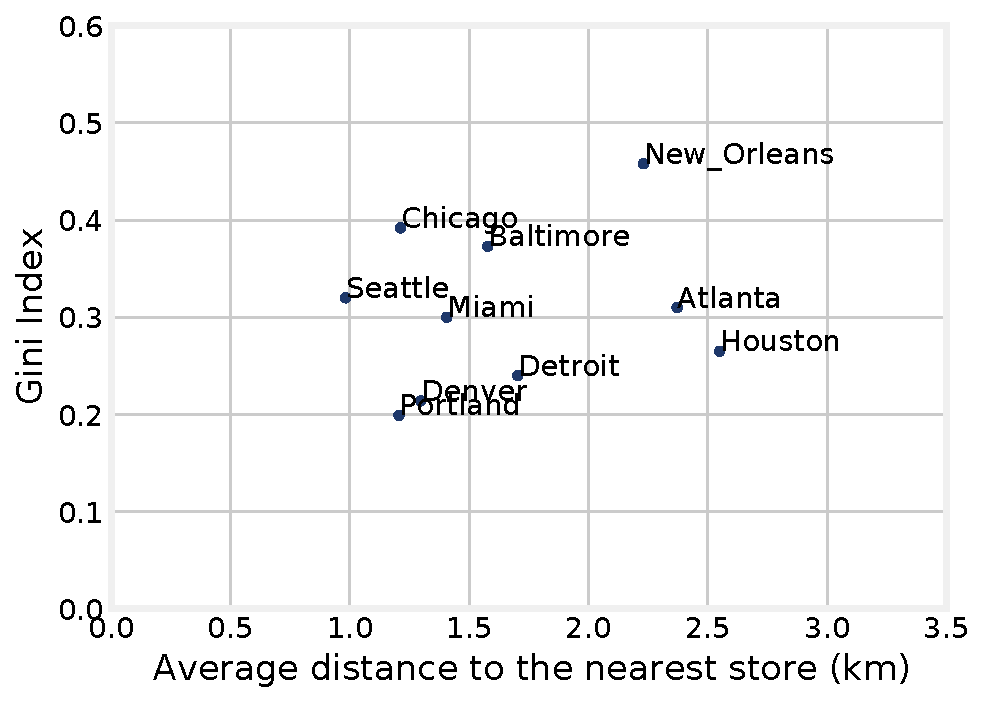
\includegraphics[width=0.9\linewidth]{report/fig/scatter_gini.pdf} 
    \end{subfigure}
    \begin{subfigure}{0.5\textwidth}
        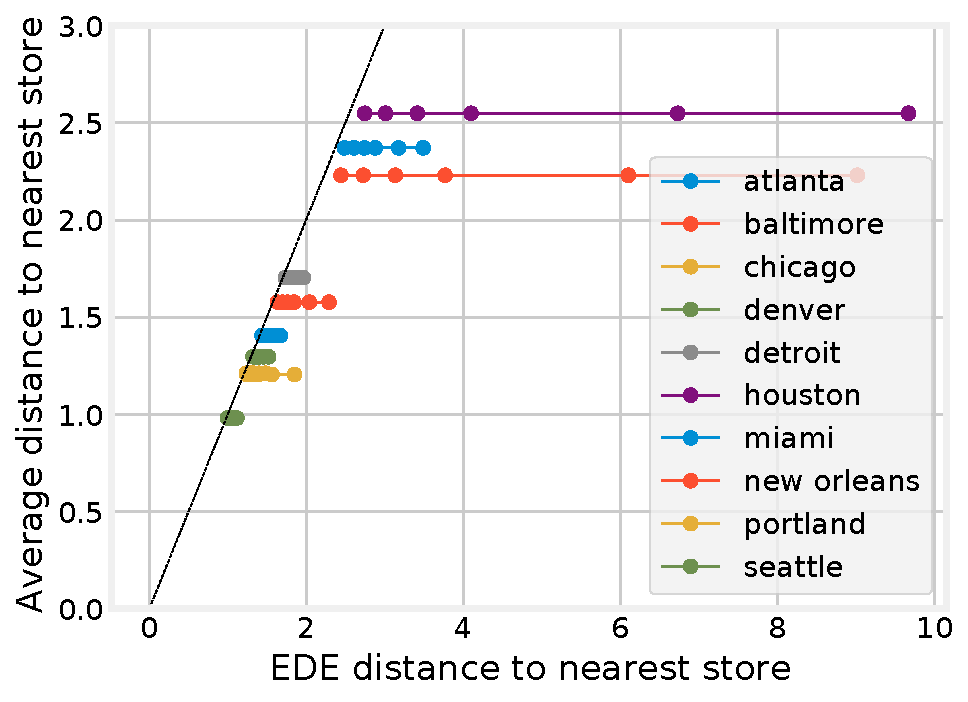
\includegraphics[width=0.9\linewidth]{report/fig/mean_ede.pdf} 
    \end{subfigure}
    \begin{subfigure}{0.5\textwidth}
        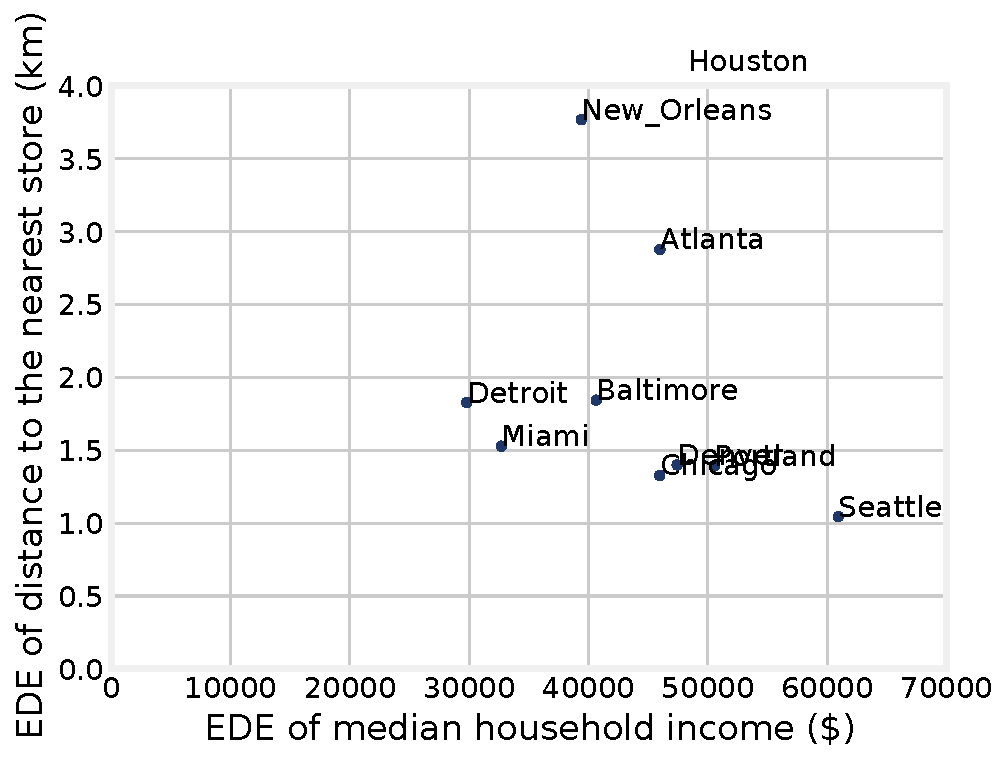
\includegraphics[width=0.9\linewidth]{report/fig/scatter_income.pdf} 
    \end{subfigure}
    \begin{subfigure}{0.5\textwidth}
        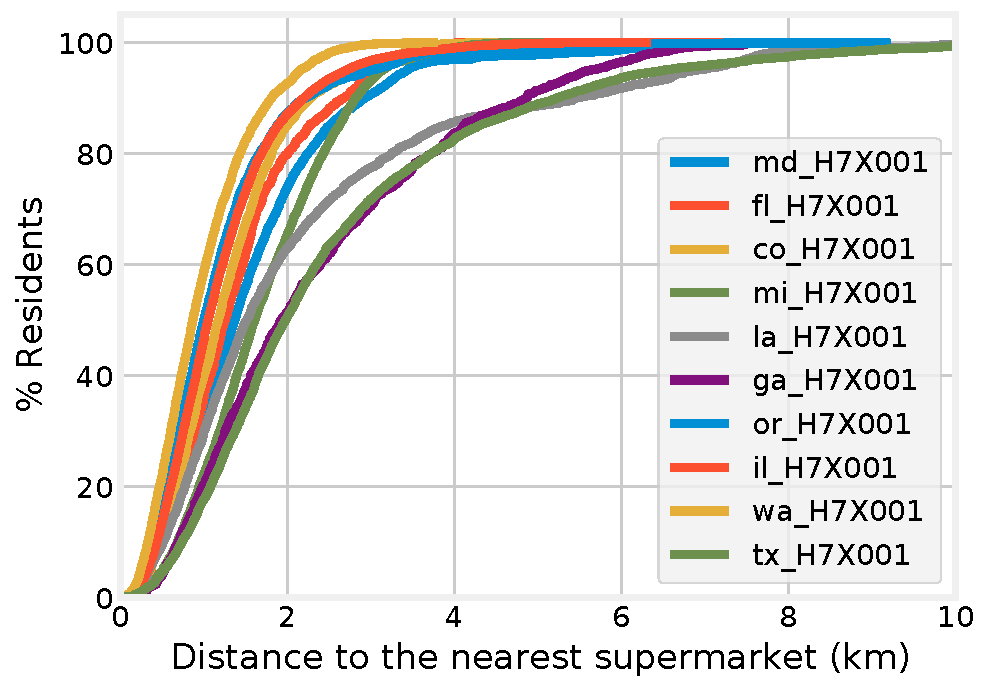
\includegraphics[width=0.9\linewidth]{report/fig/CDF_H7X001.pdf} 
    \end{subfigure}
    \caption{
    Using various approaches to measure grocery store access and its inequality in ten US cities.
    }
    \label{fig:food_deserts}
\end{figure*}

Figure \ref{fig:food_deserts}A plots each of the ten cities by their average distance to nearest grocery store against the Gini coefficient.
This is a traditional figure that shows the performance and inequality of different distributions \citep{Adger1997-tu}.
There is no correlation in this figure suggesting that, for example, although the average distance to the nearest store in Chicago is preferable, there is high \textit{relative} inequality reported.
What is unclear in this figure then is whether this is preferable to Seattle or even Houston. 
That is, would Chicago be a preferable distribution even with this relative inequality?
The challenge of using a relative inequality index is that even though the range (difference between the distance for the best-off person and the worst-off person) is smaller than the other cities, the relative index is concerned with how individuals' distances are distributed within that range.
For example, Figure \ref{fig:the_challenge} shows the distribution of Chicago and Houston: Chicago has a higher Gini coefficient even though it has a narrower distribution and is clearly provides better access to grocery stores for the residents.
However, in accessibility studies and many situations in the built environment, there is a small level of unavoidable inequality --- someone physically must live closer.
We are interested in raising the standard for all.
Clearly the Gini coefficient is not going to be particularly useful.

Figure \ref{fig:food_deserts}B plots the Kolm-Pollak EDE vs the Kolm-Pollak absolute inequality index. 
Here there is an apparent correlation and generally a clear order of preference.
We see that Chicago's general performance makes it preferable at a ``-0.5 aversion to inequality'', it also shows that at the level of aversion, the absolute inequality is actually the \textit{lowest} of all cities (no longer the second to worst). 

Figures \ref{fig:food_deserts}C and D compare the alternative measures of performance (C) and inequality (D).
In Figure \ref{fig:food_deserts}C the main concern is whether the rank ordering is similar between the measures.
The Kolm-Pollak is mathematically correct and the adjusted Atkinson follows this with the minor exception of New Orleans.
The traditional Atkinson, with inverted values, is trending in the opposite direction because a higher value is better (due to the inversion).
However, the ordering between the cities is not the same as the Kolm-Pollak, revealing one of the issues with this approach.
The mean (expected value) also follows the Kolm-Pollak, as expected, however it is not penalizing cities for inequality as the Kolm-Pollak and adjusted Atkinson do.
Figure \ref{fig:food_deserts}D is showing the inequality indices.
The Kolm-Pollak inequality index, unlike the others, is not unitless as it takes the units of the quantity evaluated.
The correlation between these indices and the Kolm-Pollak are shown in \ref{tab:compare_measures}, and there is low correlation between the Atkinson Index and the Gini coefficient, however generally strong correlation with the alternatives.

Finally, the Kolm-Pollak can be used to evaluate the performance and inequality of different demographic groups.
Figure \ref{fig:food_deserts}E shows that African Americans in almost every city evaluated are worse-off than the population as a whole and white people, with the exception of Portland (where blacks are slightly better off) and Seattle (where there is no difference). 
Figure \ref{fig:food_deserts}F shows the inequality within the demographic groups.

\subsubsection{The aversion parameter}
\label{sec:aversion}
A major component of the Kolm-Pollak method is the user-defined parameter representing aversion to inequality.
In Figure \ref{fig:aversion} we evaluate the sensitivity of the results to this parameter.
Figure \ref{fig:aversion}A presents how the Kolm-Pollak EDE changes with changing the $\beta$ (note that as $\kappa=f(\beta)$, see Equation \ref{eqn: kappa}, then $y_{EDE}=f(\beta)$).
Studying Figure \ref{fig:aversion}A and Table 2 provides insight into the behavior of the EDE.
Although $\left|\beta\right|$ is traditionally varied between 0 and 2, we plot between 0 and 10.
When $\beta=0$ the EDE is equal to the expected value of the distribution.
As $\left|\beta\right| \rightarrow \infty$ the EDE tends to the maximum value of the distribution (i.e., the value of the worst-off individual).
Consider the lines of New Orleans and Houston.
These two cities are indisputably the worst for grocery store access of the cities we evaluate.
When there is low aversion to inequality, New Orleans is preferred, because the average distance is lower.
However, as aversion to inequality is increased, New Orleans' EDE exceeds Houston.
The reason for this can be seen in how the distance is distributed between residents in Table 2.
New Orleans has a smaller distance at the 75th percentile than Houston, however, the 90th and 95th percentiles are larger.
That is, the worst-off 10\% of residents are generally worst off in New Orleans than Houston.
Although, as the maximum distance is larger in Houston, the order will switch back again as the aversion parameter tends closer to $\infty$.
Essentially, this shows that high aversion parameters make the EDE very sensitive to the values at the tail of the distribution.
Therefore, care needs to be taken when defining the boundary of a city or region (especially given the bizarre shapes of some municipalities in the USA).

Another example of the sensitivity the distribution's tail is the major change we observe for Seattle, which moves from the 2nd best to the 3rd worst as $\beta$ increases.
The reason for this is that the maximum value is significantly different to even the 95th percentile (which is second best).
In fact, the maximum value in Seattle is in fact an error in the network distance routing algorithm, which should be removed but here demonstrates the effect of an outlier on the EDE when the aversion parameter is large.
However, when the aversion parameter is less than 2, we see that the rank order is generally consistent (Figure \ref{fig:aversion}B).
When comparing different interventions (imagine these distributions are alternative interventions rather than cities) evaluating the sensitivity of rank order to the parameter provides valuable information on how much consideration is needed regarding $\beta$ (see Figure 7 in \cite{Atkinson1970-mr}).

\begin{figure*}[h!]
    % 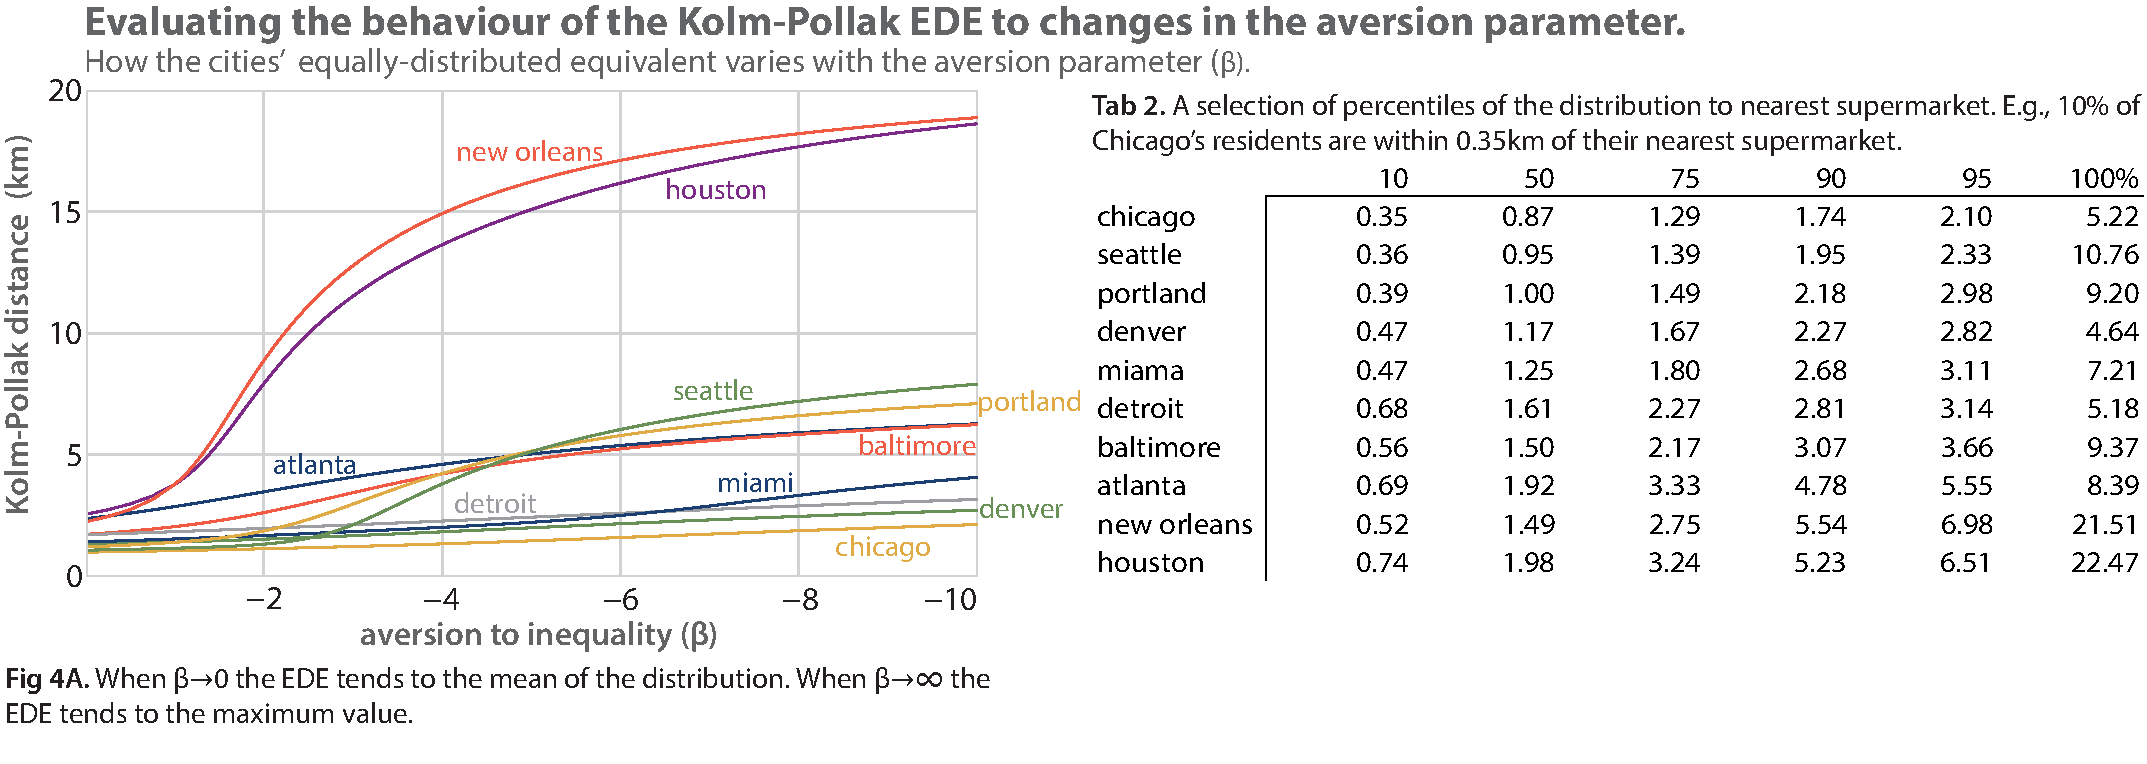
\includegraphics[width=\linewidth]{report/fig/aversion.pdf}
    \begin{subfigure}{0.5\textwidth}
        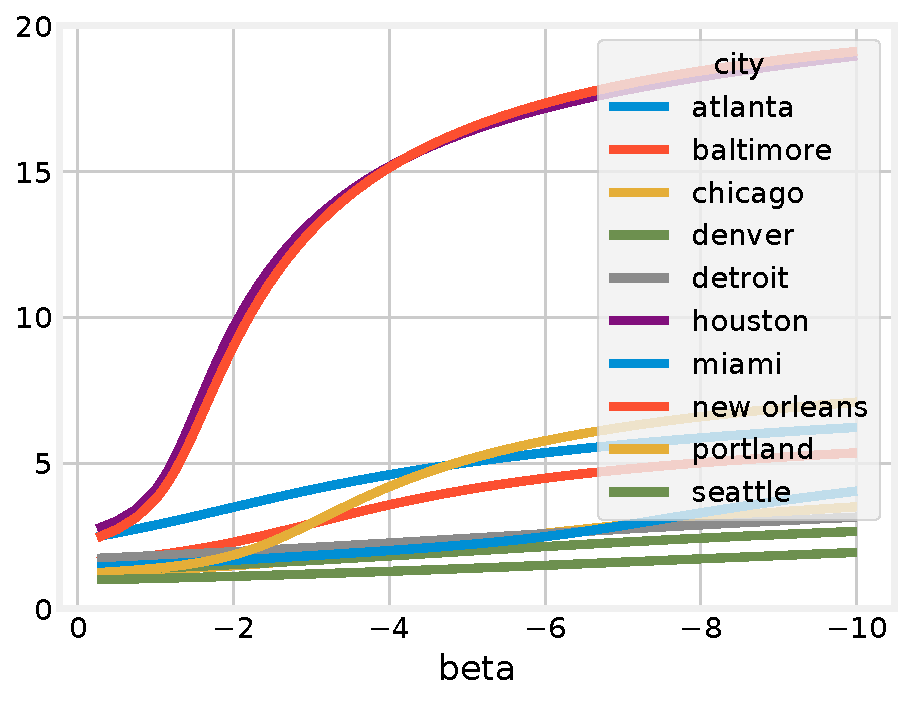
\includegraphics[width=0.9\linewidth]{report/fig/sensitivity_aversion.pdf} 
    \end{subfigure}
    \begin{subfigure}{0.5\textwidth}
        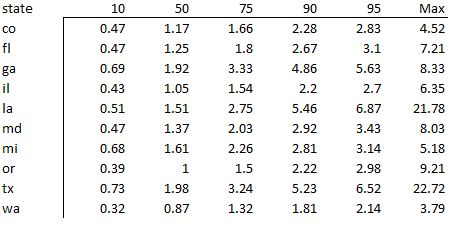
\includegraphics[width=0.9\linewidth]{report/fig/distance_percentile.JPG} 
    \end{subfigure}
    \caption{
    Evaluating the sensitivity of the Kolm-Pollak measure and inequality to the inequality aversion parameter.
    }
    \label{fig:aversion}
\end{figure*}

\subsection{Comparing socio-economic subgroups}
\begin{figure*}[]
    % \includegraphics[width=\linewidth]{report/fig/fig2.png}
    \begin{subfigure}{0.5\textwidth}
        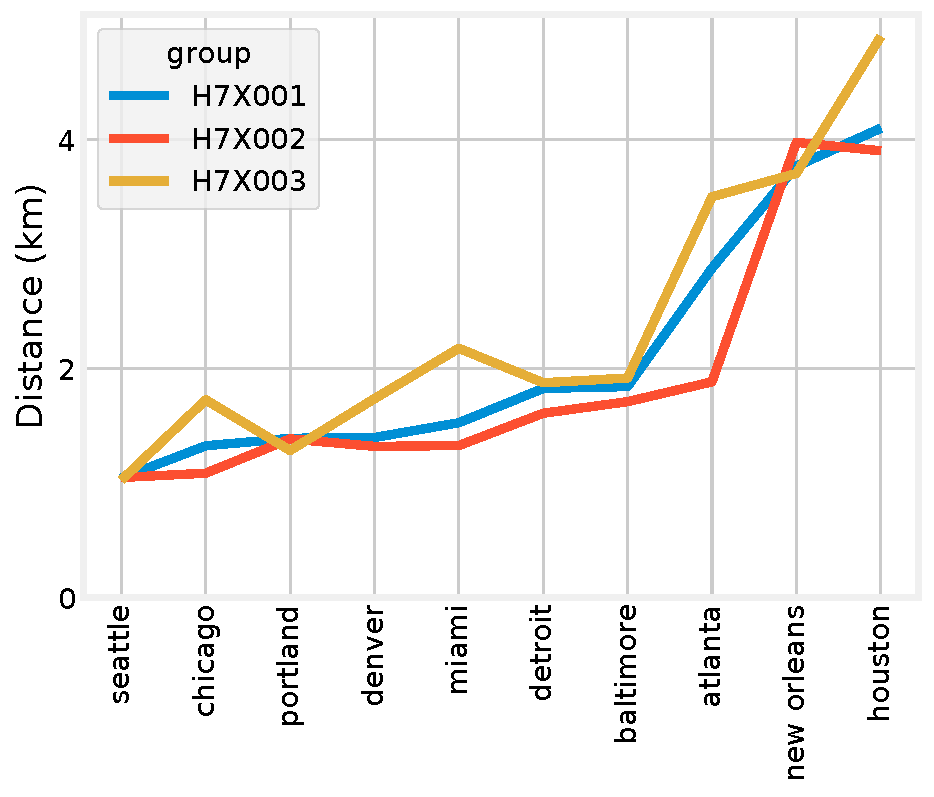
\includegraphics[width=0.9\linewidth]{report/fig/ede_subgroup_race_-1.0.pdf} 
    \end{subfigure}
    \begin{subfigure}{0.5\textwidth}
        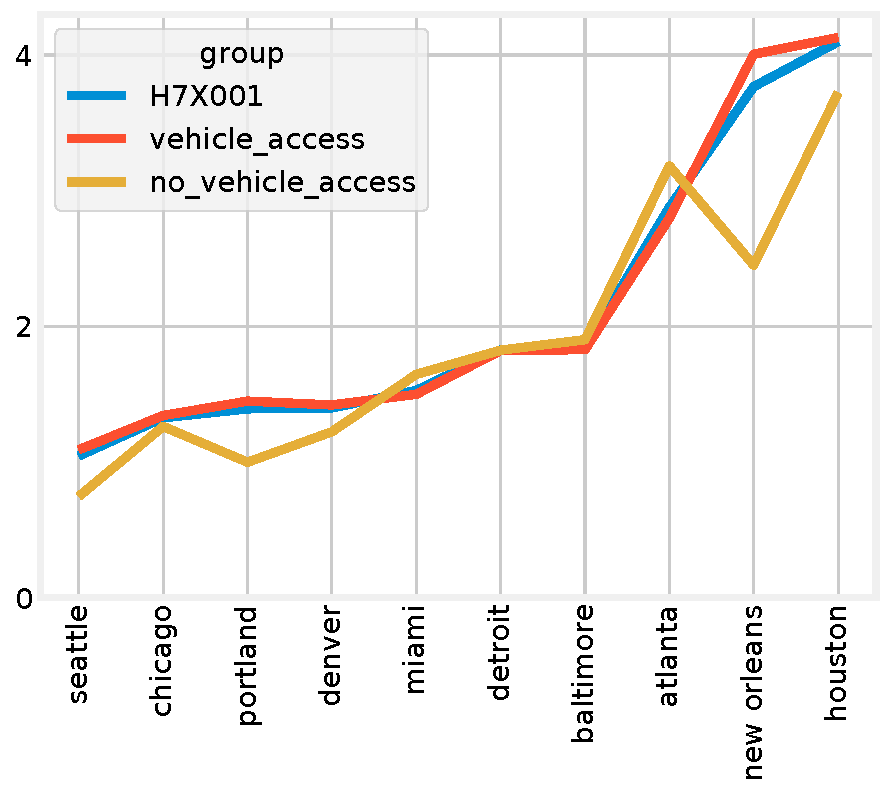
\includegraphics[width=0.9\linewidth]{report/fig/ede_subgroup_vehicle_-1.0.pdf} 
    \end{subfigure}
    \caption{
    Evaluating the performance, penalized by inequality, of different demographic and socioeconomic groups.
    }
    \label{fig:subgroup}
\end{figure*}

\subsection{Evaluating city-level planning scenarios}


\begin{figure*}[]
    % \includegraphics[width=\linewidth]{report/fig/fig2.png}
    \begin{subfigure}{0.5\textwidth}
        \includegraphics[width=0.9\linewidth]{report/fig/chicago_map_2014.pdf} 
    \end{subfigure}
    \begin{subfigure}{0.5\textwidth}
        \includegraphics[width=0.9\linewidth]{report/fig/chicago_map_2020.pdf}
    \end{subfigure}
    \begin{subfigure}{0.5\textwidth}
        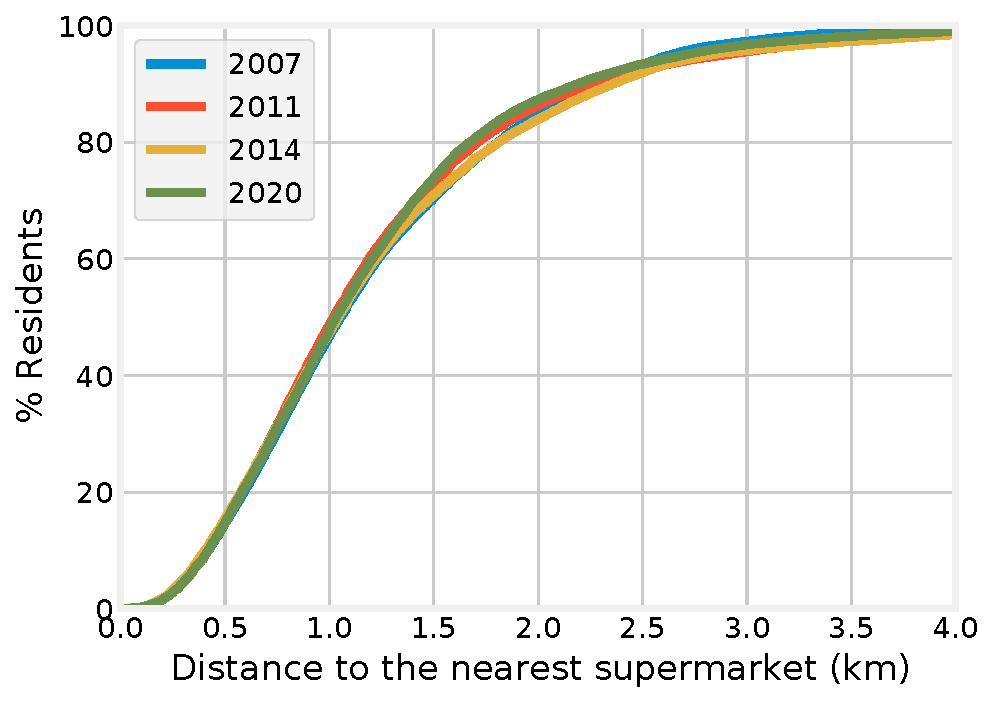
\includegraphics[width=0.9\linewidth]{report/fig/chicago_CDF_H7X001.pdf} 
    \end{subfigure}
    \begin{subfigure}{0.5\textwidth}
        % 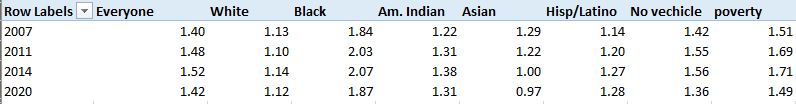
\includegraphics[width=0.9\linewidth]{report/fig/chicago_ede.JPG} 
        \begin{tabular}{lllll}
            \hline
            \textbf{}   & \textbf{2007} & \textbf{2011} & \textbf{2014} & \textbf{2020} \\ 
            \hline
            Everyone    & 1.40          & 1.48          & 1.52          & 1.42          \\
            White       & 1.13          & 1.10          & 1.14          & 1.12          \\
            Black       & 1.84          & 2.03          & 2.07          & 1.87          \\
            Am. Indian  & 1.22          & 1.31          & 1.38          & 1.31          \\
            Hisp/Latino & 1.14          & 1.20          & 1.27          & 1.28          \\
            No vechicle & 1.42          & 1.55          & 1.56          & 1.36          \\
            Poverty     & 1.51          & 1.69          & 1.71          & 1.49          \\ 
            \hline
        \end{tabular}
    \end{subfigure}
    \caption{
    How Chicago's access to supermarkets has changed over the past 13 years.
    }
    \label{fig:chicago}
\end{figure*}

\section{Discussion}
% \subsubsection{Grocery store access}
We see a strong level of agreement in the evaluations of the performance of the cities in providing access and equitable access to grocery stores.
These results show there is still significant challenges with grocery store access in many USA cities.
If the goal is to bring the city EDE's near or below 1.6km (1-mile), then only half of the ten evaluated are satisfactory (and this is given a low (-0.5) aversion to inequality).
Additionally, only three of these ten cities have an EDE less than 1.6km for African Americans, so there remains noticeable inequities in access to grocery stores.

New Orleans and Houston both have major challenges ahead to succeed in providing an acceptable and equitable level of access.
Some of their residents have extremely low access to grocery stores.

On the other hand, this study highlights remarkable progress in addressing the challenges of grocery store access.
Food deserts in Chicago were studied between 2007 and 2014 by \cite{Kolak2018-az}, who found major disparities in access; however, many of these disparities appear to have been addressed.
Although our study is not exactly comparable with \cite{Kolak2018-az}'s\footnote{\cite{Kolak2018-az} use a stricter definition of supermarket (for example, we include Aldi stores, which are not technically supermarkets due to their low product range)} there is nevertheless noticeable improvement.
These improvements demonstrate how awareness of access-deserts can successfully motivate action (e.g., city plans such as Chicago's \textit{Recipe for Healthy Places}).
Seattle's excellent access and equality between the demographic groups is another example of a success initiative to improve grocery store access.

Given the COVID-19 crisis we currently face, this access inequality places major health burdens on those without access to grocery stores.
People are forced to drive or take long public transit journeys to reach their nearest grocery store.
Having large stores that serve multiple communities, as opposed to having local stores, also increases the risk of transmission as it converges people from multiple communities to a common location.
This would be avoided with localized and walkable stores which would effectively create smaller, local communities.

Contrary to \cite{Cox2012-lg}'s criticism of inequality measures being used for environmental risks, is not that we overstate them (because the inequality of being exposed to more pollution is compensated for by lower house prices), but that we underestimate the injustices.
This method is only used for a single quantity, and enables us to discuss the inequity in (e.g., supermarket access). 
However, the challenge remains as to how we assess multiple and (worse) compounding burdens.
For example, poverty and lack of supermarket access, or poverty, lack of supermarket access, and additional amenities.
For example, in air quality (the subject of \cite{Cox2012-lg}'s criticism) this approach does not enable us to evaluate the health risk of complex mixtures of chemicals.
This highlights the importance of evaluating the distributions of environmental injustice and how we must take pains to not \textit{underestimate} these burdens or inequities.


\section{Conclusion}
The Kolm-Pollak measure provides a way of quantifying the performance and inequality of how quantities are distributed within the built environment.
This presents numerous opportunities for planners, especially with the growing interest in data-driven planning, as it enables us to evaluate the distribution of desirable and undesirable quantities and those distributions between subgroups.
While map-based visualizations are irreplaceable and will always be necessary for understanding the geographic distribution of quantities throughout a region, the EDE can be used in quantitative analysis for ranking or optimization that support decision-making, that captures inequality.
For example, where previous studies have used thresholds (e.g., ParkScore's percentage of people within 10-minute walk to nearest green space) or summary statistics in regression-type analysis, the EDE can enhance these same analysis to factor in inequality.

Practical opportunities to improve the equality of our built environment could grow following the COVID-19 crisis with the subsequent investments by governments world-wide to restart economies.
The Kolm-Pollak method enables cities to set and evaluate targets on urban characteristics, including but not limited to access to essential services. 
Policy and planning to address food-deserts and other service-deserts could foster improved, equitable access to these services which would both reduce carbon emissions and potentially improve community resilience by reducing residents' exposure to pandemics.

The Kolm-Pollak presents an opportunity for those of us working to guide decision-making in built environment contexts to reduce inequity and social injustices and ultimately enhance the  social sustainability of our communities.

\bibliography{mybibfile}

\clearpage
\newpage
\linenumbers
\appendix
%%%%%% %%%%%%%%%% %%%%%%%%%% %%%%%%%%% %%%%% SUPPLEMENTAL %%%%%%%%% %%%%%%%%%% %%%%%%%% %%%%%%%%
\section{}

\begin{table}[h]
\caption{Various metrics to evaluate a distribution and inequality indices}
\label{tab:compare_measures}
\begin{tabular}{l|RRRRRR}
\hline \hline
\multicolumn{7}{l}{\textit{Panel A. Representation of distribution (km):} $\beta=-0.5$ }\\
                                                                                   & Kolm-Pollak EDE   & Atkinson EDE   & Atkinson Adj. EDE   & Mean       & Max              &                    \\
\hline
Baltimore                                                                          & 1.85              & 0.82           & 1.89                    & 1.72       & 9.37             &                    \\
Miami                                                                              & 1.47              & 0.97           & 1.52                    & 1.41       & 7.21             &                    \\
Denver                                                                             & 1.35              & 1.02           & 1.40                    & 1.30       & 4.64             &                    \\
Detroit                                                                            & 1.77              & 0.74           & 1.80                    & 1.70       & 5.18             &                    \\
New Orleans                                                                        & 2.74              & 0.80           & 2.64                    & 2.23       & 21.51            &                    \\
Atlanta                                                                            & 2.59              & 0.63           & 2.61                    & 2.36       & 8.39             &                    \\
Portland                                                                           & 1.28              & 1.23           & 1.34                    & 1.20       & 9.20             &                    \\
Seattle                                                                            & 1.10              & 1.32           & 1.16                    & 1.07       & 10.76            &                    \\
Houston                                                                            & 2.97              & 0.62           & 2.87                    & 2.54       & 22.47            &                    \\
Chicago                                                                            & 1.02              & 1.37           & 1.07                    & 0.99       & 5.22             &                    \\

                                                                                   &                   &                &                         &            &                  &                    \\
\multicolumn{7}{l}{\textit{Panel B. Measure of inequality:} $\beta=-0.5$ }\\
                                                                                   & Kolm-Pollak Index & Atkinson Index & Atkinson Adj. Index & Gini Index & Stand. Deviation & Coef. of Variation \\
\hline
Baltimore                                                                          & 0.14              & 0.16           & 0.10                    & 0.36       & 1.18             & 0.68               \\
Miami                                                                              & 0.06              & 0.23           & 0.08                    & 0.30       & 0.82             & 0.58               \\
Denver                                                                             & 0.05              & 0.13           & 0.08                    & 0.21       & 0.74             & 0.57               \\
Detroit                                                                            & 0.06              & 0.11           & 0.06                    & 0.24       & 0.83             & 0.49               \\
New Orleans                                                                        & 0.50              & 0.22           & 0.18                    & 0.46       & 2.10             & 0.94               \\
Atlanta                                                                            & 0.23              & 0.16           & 0.11                    & 0.31       & 1.58             & 0.67               \\
Portland                                                                           & 0.08              & 0.39           & 0.12                    & 0.20       & 0.89             & 0.74               \\
Seattle                                                                            & 0.04              & 0.52           & 0.09                    & 0.32       & 0.65             & 0.61               \\
Houston                                                                            & 0.43              & 0.31           & 0.13                    & 0.26       & 1.97             & 0.78               \\
Chicago                                                                            & 0.03              & 0.17           & 0.08                    & 0.38       & 0.59             & 0.60               \\
                                                                                   & Correlation       &-0.01           & 0.88                    & 0.45       & 0.98             & 0.86               \\

\end{tabular}
\end{table}



\begin{table}[h]
\caption{Various metrics to evaluate a distribution and inequality indices}
\label{tab:compare_demographics}
\begin{tabular}{l|RRRRRR}
\hline \hline
\multicolumn{7}{l}{\textit{Panel A. Representation of distribution (km):} $\beta=-0.5$ }\\
\hline
                                                                            & Total & White & Black & Native American & Asian & Hispanic \\
Baltimore                                                                   & 1.85  & 1.67  & 1.96  & 1.82            & 1.24  & 1.70     \\
Miami                                                                       & 1.47  & 1.29  & 2.10  & 1.70            & 1.17  & 1.32     \\
Denver                                                                      & 1.35  & 1.28  & 1.66  & 1.30            & 1.38  & 1.41     \\
Detroit                                                                     & 1.77  & 1.55  & 1.82  & 1.60            & 1.35  & 1.40     \\
New Orleans                                                                & 2.74  & 2.04  & 3.13  & 2.14            & 2.57  & 2.03     \\
Atlanta                                                                     & 2.59  & 1.76  & 3.20  & 2.46            & 1.54  & 2.25     \\
Portland                                                                    & 1.28  & 1.27  & 1.22  & 1.29            & 1.46  & 1.24     \\
Chicago                                                                     & 1.02  & 0.88  & 1.29  & 0.91            & 0.77  & 0.92     \\
Seattle                                                                     & 1.10  & 1.10  & 1.10  & 1.05            & 1.11  & 1.10     \\
Houston                                                                     & 2.97  & 2.62  & 3.93  & 2.95            & 2.14  & 2.93     \\
\\
\multicolumn{7}{l}{\textit{Panel B. Measure of inequality:} $\beta=-0.5$ }\\
\hline
                                                                            & Total & White & Black & Native American & Asian & Hispanic \\
Baltimore                                                                   & 0.14  & 0.17  & 0.11  & 0.18            & 0.10  & 0.20     \\
Miami                                                                       & 0.06  & 0.04  & 0.08  & 0.07            & 0.05  & 0.04     \\
Denver                                                                      & 0.05  & 0.04  & 0.07  & 0.05            & 0.05  & 0.06     \\
Detroit                                                                     & 0.06  & 0.06  & 0.06  & 0.06            & 0.02  & 0.07     \\
New Orleans                                                                & 0.50  & 0.50  & 0.49  & 0.32            & 0.41  & 0.32     \\
Atlanta                                                                     & 0.23  & 0.10  & 0.26  & 0.24            & 0.08  & 0.21     \\
Portland                                                                    & 0.08  & 0.08  & 0.05  & 0.11            & 0.11  & 0.05     \\
Chicago                                                                     & 0.03  & 0.02  & 0.04  & 0.02            & 0.02  & 0.02     \\
Seattle                                                                     & 0.04  & 0.04  & 0.03  & 0.04            & 0.04  & 0.04     \\
Houston                                                                     & 0.43  & 0.37  & 0.56  & 0.38            & 0.17  & 0.37    
\end{tabular}
\end{table}


\clearpage
\newpage
\section{Code}
\label{appendix:code}

This is an extract of the code provided in the GitHub repository: []

\begin{lstlisting}[language=Python]
"""
Inputs:
    a = distribution of data, type=list
    weight (optional) = list of len(a)
    kappa (optional) = int < 0
    beta (optional, default = -0.5)
        if the distribution is of an undesirable (e.g., exposure)
            beta = int < 0 
        if it is a desirable property (e.g., income) 
            beta = int > 0 
    epsilon (optional, default = 0.5) = int > 0
Output:
    Kolm-Pollak EDE & Index (kappa)
    Atkinson Adjusted EDE & Index (beta)
    Atkinson EDE & Index (epsilon)
    Gini Index
"""

import numpy as np
from scipy.integrate import simps

def kolm_pollak_ede(a, beta = None, kappa = None, weight = None):
    """returns the Kolm-Pollak EDE"""
    a = np.asanyarray(a)

    if kappa is None:
        if beta is None:
            raise TypeError("you must provide either a beta or kappa aversion parameter")
        kappa = calc_kappa(a, beta, weight)

    if weight is None:
        ede_sum = np.exp(a*-kappa).sum()
        N = len(a)
    else:
        ede_sum = np.multiply(np.exp(a*-kappa), weight).sum()
        N = sum(weight) # for a weighted average

    ede = (-1 / kappa) * np.log(ede_sum / N)
    return(ede)


def kolm_pollak_index(a, beta = -0.5, kappa = None, weight = None):
    """returns the Kolm-Pollak Inequality Index"""
    if weight is None:
        x_mean = np.mean(a)
    else:
        x_mean = np.average(a, weights = weight)

    a = a - x_mean

    inequality_index = kolm_pollak_ede(a, beta = beta, kappa = kappa, weight = weight)

    return(inequality_index)

\end{lstlisting}

\section{}
\label{appendix: measures}
    
\subsubsection{Atkinson EDE}
As a comparison, we also use the Atkinson EDE and index \citep{Atkinson1970-mr}.
The Atkinson approach is suitable for distributions of desirable quantities, but mathematically unsuited for distributions of undesirable quantities.
This is because it is constructed to prioritize individuals with low values of the quantity (e.g., the poor when considering wealth).
This can be slightly ameliorated by considering the inverse of the quantity (e.g., $\frac{1}{\textrm{distance}}$ instead of distance, where small distance is preferable). 
However, when comparing alternatives the rank order changes between the quantity and its complement, rendering this approach unsuitable. 
Nevertheless, as it is not uncommonly used we include it here. 
The Atkinson EDE can be calculated using
\begin{equation}
    y_{EDE_A} = \left[ \frac{1}{N}\sum_{i=1}^N 
    \left( \frac{1}{x_i}
   \right) ^{1-\beta}\right]^{\frac{1}{1-\beta}} 
\end{equation}
Where $\beta > 0$.

Alternatively, the Adjusted Atkinson EDE could be calculated \citep{Sheriff2020-ge} as 
\begin{equation}
    y_{EDE_{A'}} = \left[ \frac{1}{N} \sum_{i=1}^N x_i^{1-\beta}\right]^{\frac{1}{1-\beta}}
\end{equation}
Where, in this case, $\beta < 0$ and the values are not be inverted.

The two inequality indices respectively are
\begin{equation}
    I_A = 1 - \frac{y_{EDE_A}}{E[X]}
\end{equation}
Where $E[X]$ = the mean or expected value of $X$.
\begin{equation}
    I_{A'} = \frac{y_{EDE_{A'}}}{E[X]} -1
\end{equation}
Unlike the Kolm-Pollak inequality index, these are relative inequality indices.

\subsubsection{Gini Index}
The Gini coefficient is the most commonly used inequality index \citep{Maguire2011-fi}.
It is derived from the Lorenz curve which is constructed by plotting cumulative values along the $x$ axis with cumulative density on the $y$ axis. 
Once the curve has been produced, the Gini index is calculated by dividing the area between the curve and the diagonal line that would represent equality, by the total area under the equality line.
\begin{equation}
    G = \frac{A_{equality}-A_{observed}}{A_{equality}}
\end{equation}

\subsubsection{Coefficient of Variation}
The coefficient of variation is a more conventional summary statistic.
It measures the relative dispersion or spread of a data, normalized by the mean of the data: 
\begin{equation}
    CV = \frac{\sigma}{\mu}
\end{equation}
Where
\begin{conditions}
     \sigma & standard deviation\\
     \mu & mean \\   
\end{conditions}


\end{document}

